
\chapter{极坐标与参数方程}

\section{极坐标系与曲线的极坐标方程}
\subsection{极坐标的概念}

如果知道了一点相对于一定点的距离和方向,那么这个
点的位置就被唯一确定了.这就是说,我们可用角度和距离
来确定平面上点的位置.这节,我们研究如何利用角度和距
离来建立坐标系.

在平面内取一个定点$O$, 叫做\textbf{极点},引射线$OA$, 叫做
\textbf{极轴},再选定一个长度单位和角度的正向(通常取逆时针方
向).对于平面上任一点$P$, 但$P$不是极点,用$r$表示$\overline{OP}$
的长度,$\theta$表示从$OA$转到$OP$的角度.这时$r$叫做$P$点的
\textbf{极径},$\theta$叫做$P$点的\textbf{极角}.有序实数对$(r,\theta)$就叫做$P$点
的极坐标,并记作$P(r,\theta)$. 这样建立的坐标系叫做极坐
标系(图7.1).

在极坐标系中,$r=0$,
不论$\theta$是什么角,$(0,\theta)$
都表示极点,除去极点,显
然,不同的点对应不同的极
坐标;反过来任取一对实数
$(r,\theta)$, 其中$0<r<\infty$, $0\le 0\theta<2\pi$, 我们能够且只能够
在平面上找到一点$P$, 使它的坐标恰好是$(r,\theta)$. 由此可
见,平面上除了极点外的所有点和实数对集合:
\[\{(r,\theta)|0<r<\infty,\quad 0\le\theta<2\pi\}\]
可建立一一对应关系.

有时为了研究问题的需要,我们往往取消上述对$r,\theta$
的限制,规定$r$和$\theta$可取任何实数值.如果已知任意有序实
数对$(r,\theta)$, 那么,我们可按下面的方法,在极坐标系中
作出它的对应点.

\begin{figure}[htp]\centering
    \begin{minipage}[t]{0.48\textwidth}
    \centering
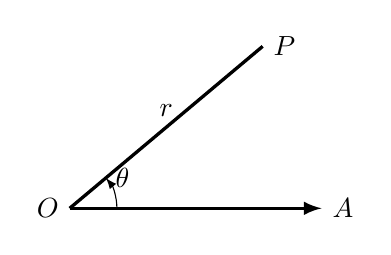
\begin{tikzpicture}[>=latex, scale=.8]
\draw[->, very thick](0,0)node[left]{$O$}--(4,0)node[right]{$A$}; 
\draw[very thick](0,0)--node[above]{$r$}(40:4)node[right]{$P$};
\draw[->](.75,0) arc (0:40:.75)node[right]{$\theta$};
\tkzDrawPoint(40:4)
    \end{tikzpicture}
    \caption{}
    \end{minipage}
    \begin{minipage}[t]{0.48\textwidth}
    \centering
    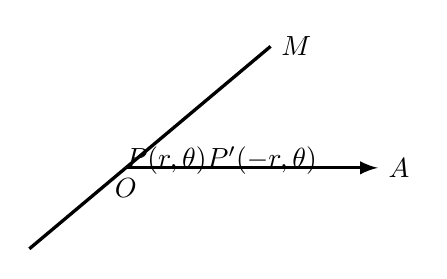
\begin{tikzpicture}[>=latex, scale=.8]
\draw[->, very thick](0,0)node[below]{$O$}--(4,0)node[right]{$A$}; 
\draw[very thick](0,0)--(40:3)node[right]{$M$};
\draw[very thick](0,0)--(-180+40:2);
\tkzDefPoint(40:1.5){P}
\tkzDefPoint(-180+40:1.5){P'}
\tkzDrawPoints(P,P')
\tkzLabelPoint[right=2pt](P){$P(r,\theta)$}
\tkzLabelPoint[right=2pt](P'){$P'(-r,\theta)$}
    \end{tikzpicture}
    \caption{}
    \end{minipage}
    \end{figure}


以极轴$OA$为始边,作有向角$\angle AOM=\theta$, 如果$r>0$, 
在射线$OM$上作$\overline{OP}=r$, 
如果$r<0$, 在射线$OM$的反
向延长线上作$\overline{OP}=|r|$. 这
样,对任一对有序实数$(r,\theta)$,我们总可以在平面上
确定一点$P$; 反过来,对平
面上任一点$P$, 都可对应无限多有序实数对组成的极坐标,
如果已知$P(r,\theta)$, 那么$(r,\theta+2k\pi)$, 当$k$为任意整数
时,都可表示$P$点的极坐标.

\begin{example}
    在极坐标系中,作出下列各点
\[B\left(4,\frac{\pi}{6}\right),\qquad C(2,0),\qquad D\left(4,\frac{5}{6}\pi\right),\qquad E\left(4,\frac{3}{2}\pi\right)\]
\[F\left(-4,\frac{\pi}{6}\right),\qquad G\left(3,-\frac{\pi}{3}\right),\qquad H\left(1,\frac{\pi}{2}\right)\]
\end{example}

\begin{solution}
    如图7.3所示.
\begin{figure}[htp]
    \centering
\begin{tikzpicture}[>=latex, scale=.7]
\draw[->, thick](0,0)--(5,0)node[right]{$A$};
\foreach \x in {1,2,3,4}
{
    \draw(0,0) circle(\x);
}    
\foreach \x in {30,90,...,330}
{
    \draw(0,0)--(\x:5);
}
\tkzDefPoint(30:4){B}
\tkzDefPoint(0:2){C}
\tkzDefPoint(150:4){D}
\tkzDefPoint(270:4){E}
\tkzDefPoint(30:-4){F}
\tkzDefPoint(-60:3){G}
\tkzDefPoint(90:1){H}
\tkzDefPoints{0/0/O}
\tkzDrawPoints(B,C,D,E,F,G,H)
\tkzAutoLabelPoints[center=O](G)
\node at (O)[below left]{$O$};
\tkzLabelPoints[above right](C,H,E)
\tkzLabelPoints[above](D,B)
\tkzLabelPoints[left](F)
\end{tikzpicture}   
    \caption{}
\end{figure}
\end{solution}

\begin{ex}
\begin{enumerate}
    \item 在极坐标系中,描出下各点.
  \[  L\left(3,\frac{\pi}{3}\right),\qquad  M(3,0),\qquad N\left(1,\frac{\pi}{2}\right),\qquad P\left(-3,\frac{\pi}{4}\right)\]
\[    Q\left(3, -\frac{\pi}{4}\right), \qquad R\left(-2,-\frac{2}{3}\pi\right),\qquad S\left(1,\frac{3}{4}\pi \right)\]
\item 在极坐标系中,描出下列各点和它们关于原点和极轴的
    对称点.
\[P_1\left(2,\frac{\pi}{3}\right),\qquad P_2\left(-3,\frac{\pi}{2}\right),\qquad P_3\left(\frac{5}{4},\frac{\pi}{4}\right)\]
    \item 已知一等边三角形边长为$a$, 它的中心与极点重合,一
    个顶点在极轴上,求三个顶点的极坐标.
    \item 已知一正方形边长是$2a$, 它的中心在极点,它的一边与
    极轴垂直.求它的四个顶点的极坐标.
\end{enumerate}
\end{ex}

\subsection{极坐标和直角坐标的关系}

\begin{figure}[htp]
    \centering
\begin{tikzpicture}[>=latex]
    \draw[-> ](-.5,0)--(4,0)node[right]{$X$};
    \draw[-> ](0,-.5)--(0,2.5)node[right]{$Y$};
\draw(0,0)node[below left]{$O$}--node[left]{$r$}(30:3)node[above]{$P$}--node[right]{$y$}+(0,-1.5);
\node at (1.5,0)[below]{$x$};
\draw(.6,0) arc(0:30:.6)node[right]{$\theta$};
\end{tikzpicture}
    \caption{}
\end{figure}

在平面上建立一直角坐标系$OXY$和一极坐标系,使极
点和坐标原点$O$重合,极轴$OA$与$X$轴的正半轴重合.设平
面上任一点$P$在$OXY$中的
坐标为$(x,y)$, 在极坐
标系中的坐标为$(r,\theta)$. 
若$P$点的极坐标为已知,且$r>0$, 则由三角学可知,
$P$点的直角坐标可由变换公式
\begin{equation}
    x=r\cos\theta,\qquad y=r\sin\theta
\end{equation}
求得.若$r=0$, 公式(7.1)显然成立,若$r<0$, 则因
$(r,\theta)$和$(-r,\theta+\pi)$表示同一点,故可用$(-r,\theta+\pi)$
代替$(r,\theta)$来求$(x,y)$, 于是
\[\begin{split}
    x&=-r\cos(\theta +\pi )=-r(-\cos\theta )=r\cos\theta \\
    y&=-r\sin(\theta +\pi )=(-r)(-\sin\theta )=r\sin\theta 
\end{split}\]
因此,当$r<0$时,点的直角坐标仍可由公式(7.1)求得.

反过来,如果$P$点的直角坐标为已知,我们可由公式
\begin{equation}
    r^2=x^2+y^2,\qquad \tan\theta=\frac{y}{x}\quad (x\ne 0)
\end{equation}
求得该点的极坐标,由上一小节可知,点$P$的极坐标可对应
无穷多对数值,其中任一对数值都可作为点$P$的极坐标.在
一般情况下,我们只求$r\ge 0$, $0\le 0<2\pi$ 的一对数值就可
以了.

\begin{example}
    把点$P$的极坐标$\left(3,\frac{\pi}{3}\right)$化为直角坐标.
\end{example}

\begin{solution}
    由于
\[\begin{split}
    x&=3\cdot \cos \frac{\pi}{3}=3\cdot \frac{1}{2}=\frac{3}{2}\\
    y&=3\cdot \sin \frac{\pi}{3}=3\cdot \frac{\sqrt{3}}{2}=\frac{3\sqrt{3}}{2}\\
\end{split}\]
因此:点$P$的直角坐标是$\left(\frac{3}{2},\frac{3\sqrt{3}}{2}\right)$
\end{solution}

\begin{example}
    把点$M(-1,-1)$化为极坐标.
\end{example}

\begin{solution}
\[\begin{split}
    r&=\sqrt{(-1)^2+(-1)^2}=\sqrt{2}\\
    \tan\theta&=\frac{-1}{-1}=1
\end{split}\]
由于点$M$在第三象限.因此,取$\theta=\frac{5\pi}{4}$

$\therefore\quad $点$M$的极坐标为$\left(\sqrt{2},\frac{5}{4}\pi\right)$
\end{solution}

\begin{ex}
\begin{enumerate}
    \item 试求下列各点的直角坐标.
\[M\left(-4,-\frac{\pi}{4}\right),\qquad N\left(-4,-\frac{5}{4}\pi\right),\qquad P(-3,8\pi)\]
\[Q(7,0^{\circ}),\qquad R\left(5,-\frac{\pi}{2}\right),\qquad S\left(-2,-\frac{2}{3}\pi\right)\]
    \item 试求下列各点的极坐标.
\[B(1,-1),\qquad C\left(3,\sqrt{3}\right),\qquad D(-1,1)\]
\end{enumerate}
\end{ex}

\subsection{点的轨迹的极坐标方程}
我们已知,可用一对有序实数$(r,\theta)$来确定平面上
一点的位置,因此,平面上点的轨迹有时可用含有$r,\theta$两个
变量的方程来表示,这个方程叫做点的轨迹的\textbf{极坐标方程}或
简称\textbf{极方程}.


\begin{example}
    求通过极点$O$且与极轴成定角$\alpha$的直线的极坐标
    方程(图7.5).
\end{example}

\begin{solution}
    设点$P(r,\theta)$为已知直线上的任一点,则点$P$
    满足极方程
 \begin{equation}
     \theta=\alpha
 \end{equation}
    反之,对任一实数$r$, 以$(r,\alpha)$为极坐标的点也一定满
    足方程(7.3). 因此方程(7.3)就是所求的直线的极方程.
\end{solution}

\begin{figure}[htp]\centering
    \begin{minipage}[t]{0.48\textwidth}
    \centering
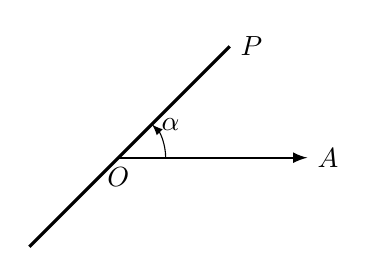
\begin{tikzpicture}[>=latex, scale=.8]
    \draw[->, thick](0,0)node[below]{$O$}--(3,0)node[right]{$A$}; 
    \draw[very thick](0,0)--(45:2.5)node[right]{$P$};
    \draw[very thick](0,0)--(-180+45:2);
\draw[->](.75,0) arc (0:45:.75)node[right]{$\alpha$};

    \end{tikzpicture}
    \caption{}
    \end{minipage}
    \begin{minipage}[t]{0.48\textwidth}
    \centering
    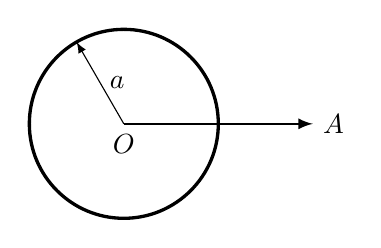
\begin{tikzpicture}[>=latex, scale=.8]
\draw[->, thick](0,0)node[below]{$O$}--(3,0)node[right]{$A$};
\draw[very thick](0,0) circle (1.5); 
\draw[->](0,0)--node[right]{$a$}(120:1.5);
    \end{tikzpicture}
    \caption{}
    \end{minipage}
    \end{figure}

\begin{example}
    求圆心在极点$O$, 半径为$a$的圆的极坐标方程
(图7.6).
\end{example}

\begin{solution}
    因为对任一点$P(r,\theta)$,当且仅当
\begin{equation}
    r=a
\end{equation}
时,$P$点才在已知圆上,所以(7.4)式就是所求圆的极方程.
\end{solution}

\begin{example}
    试求以$C(a,0)$为圆心,以$a$为半径的圆的
    极坐标方程(图7.7). 
\end{example}

\begin{figure}[htp]
    \centering
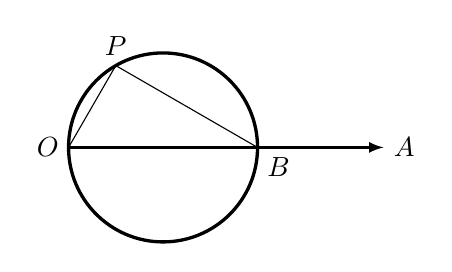
\begin{tikzpicture}[>=latex, scale=.8]
\draw[->, thick](0,0)--(5,0)node[right]{$A$};
\draw[very thick](1.5,0) circle (1.5); 
\draw (0,0)node[left]{$O$}--(60:1.5)node[above]{$P$}--(3,0)node[below right]{$B$};
\tkzDefPoint(1.5,0){C}
\tkzDrawPoint(C)
\tkzLabelPoints[below](C)
    \end{tikzpicture}
    \caption{}
\end{figure}

\begin{solution}
    由已知条件,圆心在
极轴上,圆经过极点$O$. 设圆
和极轴的另一个交点是$B$. 得
知$P(r,\theta)$在已知圆上的充要条件是$\angle OPB=\pi/2$, 即
\[|\Vec{OP}|=|\Vec{OB}|\cos\theta\]
\begin{equation}
    r=2a\cos\theta
\end{equation}
因此(7.5)式就是所求圆的极方程.
\end{solution}

如果某动点的轨迹在直角坐标系中的方程为已知,那
么,利用变换公式
\[x=r\cos\theta,\qquad y=r\sin\theta\]
可求得该动点轨迹的极坐标方程;反之,若一动点的轨迹的
极方程为已知,我们也可用上节变换公式(7.2), 把它化为
在直角坐标系中的方程.

\begin{example}
    设一圆的方程为
\[x^2+y^2-8y=0\]
如果以原直角坐标系的原点为极点,$X$轴的正半轴为极轴,
求这圆的极方程.
\end{example}

\begin{solution}
    将$x=r\cos\theta$, $y=r\sin\theta $, 代入已知圆的方程,得
\[r^2-8r\sin\theta =0\]
即$r=8\sin\theta$.
这就是已知圆的极坐标方程.
\end{solution}

\begin{example}
    已知直线的极方程为$r\sin\theta=2$, 把它化为直角
    坐标方程.
\end{example}

\begin{solution}
    将$r=\sqrt{x^2+y^2}$, $\sin\theta =\frac{y}{r}$代入已知直线的极方
程,得
\[\sqrt{x^2+y^2}\cdot \frac{y}{\sqrt{x^2+y^2}}=2\]
即
$y=2$. 
这就是已知直线的直角坐标方程.
\end{solution}

我们可根据极方程用描点法近似地作出这个极方程的图
象,下面举例说明.

\begin{example}
    描出方程$r=a\theta\; (a>0)$的图象.
\end{example}

\begin{solution}
    与直角坐标系中的作图步骤一样,先给出$\theta$一系列
的允许值,算出$r$的对应值,由此得到一对应值表.然后再
根据对应值表描点作图(图7.8).
\begin{center}
\begin{tabular}{c|cccccccccc}
\hline
$\theta$ & 0&$\frac{\pi}{4}$&$\frac{\pi}{2}$&$\frac{3\pi}{4}$&$\pi$&$\frac{5\pi}{4}$&$\frac{3\pi}{2}$&$\frac{7\pi}{4}$&$2\pi$&$\cdots$\\
\hline
$r$ & 0&  $0.78a$ & $1.57a$ & $2.36a$ & $3.14a$ & $3.93a$ & $4.71a$ & $5.50a$ & $6.28a$ & $\cdots$\\
\hline
\end{tabular}
\end{center}
\begin{figure}[htp]
    \centering
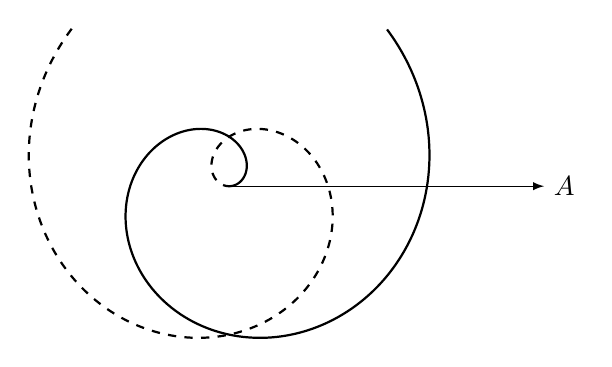
\begin{tikzpicture}[>=latex, scale=.8]
    \draw[->](0,0)--(5,0)node[right]{$A$};
\draw[domain=0:2.25*pi, samples=1000, thick]plot({\x r}: {.5*\x});
\draw[domain=-2.25*pi:0, samples=1000, thick, dashed]plot({\x r}: {.5*\x});
\end{tikzpicture}
    \caption{}
\end{figure}

方程$r=a\theta,\; (a>0)$的图象,叫做\textbf{阿基米德螺线}.
\end{solution}

\begin{ex}
\begin{enumerate}
    \item 求通过极点$O$且与极轴$OA$成$\pi/6$
    角的直线的极方程.
    \item 求以$C(3,\pi/3)$
    为圆心,半径等于2的圆的极方程.
    \item 求通过点$P(r,\theta )$且与原点距离等于$d$的直线的极方
    程.
    \item 求$M(r_1,\theta_1)$, $N(r_2,\theta_2)$两点间的距离.
    \item 把下列直角坐标方程化为极方程.
\begin{multicols}{2}
\begin{enumerate}
\item $x=6$
\item $y=2x$
\item $x^2+y^2-9=0$
\item $x^2+y^2-4x+8=0$
\item $xy=4$
\item $x^2-y^2=1$
\item $y^2=4x$
\item $(x^2+y^2)^2=a^2(x^2-y^2)$
\end{enumerate}
\end{multicols}

    \item 把下列极坐标方程,化为直角坐标方程.
\begin{multicols}{2}
\begin{enumerate}
\item $r=3$
\item $\theta=\frac{\pi}{4}$
\item $r=3\cos\theta$
\item $r=5\tan\theta$
\item $r^2\cos 2\theta=16$
\item $r=\frac{6}{1+2\cos\theta}$
\end{enumerate}
\end{multicols}
    \item 画出心脏线$r=a(1+\cos\theta )$的图象.
    \item 画出双纽线$p^2=a^2\cos2\theta$的图象.
\end{enumerate}
\end{ex}

\subsection{圆锥曲线的极坐标方程}
在第六章中,我们给圆锥曲线下了一个统一的定
义,现在我们根据这个定义来求圆锥曲线统一的极方程.

已知圆锥曲线的焦点$F$和准线$\ell$, 过$F$作$\ell$的垂线,设
垂足为$D$. 以$F$为极点,$\Vec{DF}$的方向作为极轴的方向建立极
坐标系(图7.9).设$P(r,\theta)$是曲线上任一点,作$\overline{PF}$, 
再作$PQ\bot\ell$, $PM$垂直极轴,垂足分别为$Q,M$. 设$F$到
准线$\ell$的距离$\overline{FD}=p$, 则由圆锥曲线的定义,得
\[\frac{PF}{PQ}=e\]
即:$r=e\cdot PQ$

$\because\quad PQ=DF+r\cos\theta=p+r\cos\theta$

$\therefore\quad r=e(p+r\cos\theta)$

解出$r$,得:
\begin{equation}
\boxed{ r=\frac{ep}{1-e\cos\theta}}   
\end{equation}

这就是圆锥曲线的极方程.当$0<e<1$时,方程(7.6)
表示椭圆,定点$F$是它的左焦点,定直线$\ell$是它的左准线;
当$e=1$时,方程(7.6)表示开口向右的抛物线;当$e>1$
时,方程(7.6)表示双曲线,定点$F$是它的右焦点,定直线
$\ell$是它的右准线(图7.10).

\begin{figure}[htp]\centering
    \begin{minipage}[t]{0.48\textwidth}
    \centering
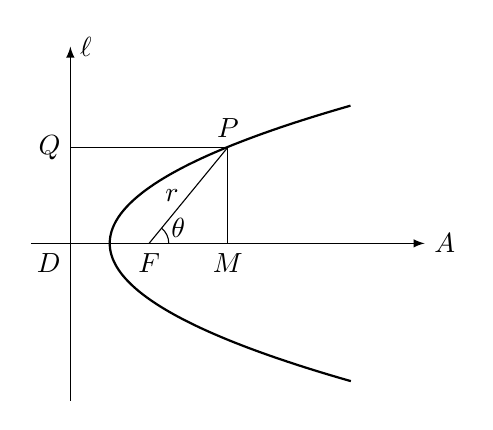
\begin{tikzpicture}[>=latex, scale=1]
    \draw[->](-1,0)--(4,0)node[right]{$A$};
    \draw[->](-.5,-2)--(-.5,2.5)node[right]{$\ell$};
    \draw[domain=-1.75:1.75, samples=100, thick] plot({\x*\x}, \x);
    \draw(1.5,0)node[below]{$M$}--(1.5,1.22)node[above]{$P$}--(-.5,1.22)node[left]{$Q$};        
    \draw(.5,0)node[below]{$F$}--node[left]{$r$}(1.5,1.22);
\draw(.75,0) arc (0:50.77:.25)node[right]{$\theta$};
\node at (-.5,0)[below left]{$D$};
    \end{tikzpicture}
    \caption{}
    \end{minipage}
    \begin{minipage}[t]{0.48\textwidth}
    \centering
    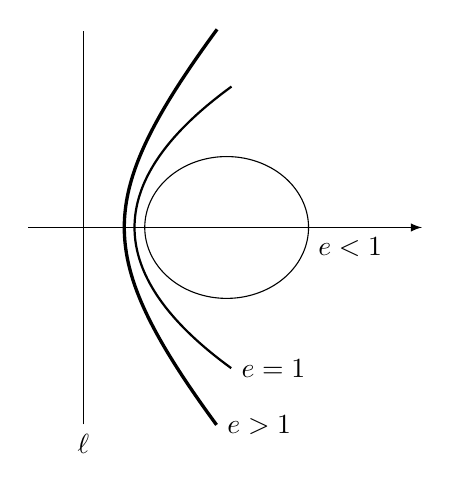
\begin{tikzpicture}[>=latex, scale=1]
\draw[->](-2,0)--(3,0);
\draw(-1.3,-2.5)node[below]{$\ell$}--(-1.3,2.5);
\draw[domain=0:2*pi, samples=300]plot({\x r}: {.6*1.3/(1-.5*cos(\x r))})node[below right]{$e<1$};
 \draw[domain=0.4*pi:1.6*pi, samples=300, thick]plot({\x r}: {1*1.3/(1-1*cos(\x r))})node[right]{$e=1$};
\draw[domain=0.45*pi:1.55*pi, samples=300, very thick]plot({\x r}: {1.5*1.3/(1-1.5*cos(\x r))})node[right]{$e>1$};
    \end{tikzpicture}
    \caption{}
    \end{minipage}
    \end{figure}

\begin{ex}
\begin{enumerate}
    \item 求证圆锥曲线$r=\frac{ep}{1-e\cos\theta}$,
    当$0<e\le 1$时的直角
    坐标方程是
    \[(1-e^2)x^2+y^2-2e^2px-e^2p^2=0\]
    当$e>1$时,直角坐标方程是$\sqrt{x^2+y^2}=e(x+p)$.
    \item 一颗慧星的轨道是抛物线,太阳位于这条抛物线的焦点
    上,已知这颗慧星在距太阳为$1.6\x10^8$公里时,它的极
    径和轨道轴成$60^{\circ}$角.求这颗慧星的轨道的极方程,并
    且求出它的近日点与太阳的距离.
    \item 说明下列方程的图形是什么,并且画出草图.
\begin{multicols}{2}
    \begin{enumerate}
        \item $r=\frac{5}{1-\cos\theta}$
        \item $r=\frac{5}{3-4\cos\theta}$
        \item $r=\frac{1}{2-\cos\theta}$
        \item $r=\frac{4}{1+\cos\theta}$
    \end{enumerate}
\end{multicols}
\end{enumerate}
\end{ex}

\section*{习题7.1}
\addcontentsline{toc}{subsection}{习题7.1}

\begin{enumerate}
    \item 作出下列极方程的图象,并说明它们各是什么曲线.
\begin{multicols}{2}
    \begin{enumerate}
        \item $r=1$
        \item $\theta=\frac{\pi}{3}$
        \item $r\cos\theta =2$
        \item $r\sin\theta =1$
        \item $r=6\cos\theta$
        \item $r=10\sin\theta$
    \end{enumerate}
\end{multicols}

    \item 求满足下列条件的各图形的极方程.
\begin{enumerate}
 \item 经过点$P\left(2,\frac{\pi}{4}\right)$, 
    垂直于极轴的直线;
    \item 经过点$Q\left(3,\frac{\pi}{3}\right)$, 
    平行于极轴的直线;
    \item 圆心在极点,半径等于$a$的圆;
    \item 圆心在点$B\left(a,\frac{\pi}{2}\right)$
    半径等于3的圆;
    \item 圆心在$C(a,\pi)$, 半径等于$a$的圆;
    \item 经过点$P(a,0)$和极轴相交成$\alpha$角的直线.  
\end{enumerate}

    \item 从极点作圆$r=2a\cos\theta$的各弦,求各弦中点的轨迹的极
    坐标方程.
    \item 从极点$O$作直线和直线$r\cos\theta=4$相交于$M$点,在$\overline{OM}$
    上取一点$P$, 使$\overline{OM}\cdot\overline{OP}=12$, 求$P$点轨迹的极坐标
    方程.
    \item 求适合于下列条件的轨迹的极坐标方程,并且画出轨迹
    的草图.
\begin{enumerate}
    \item 点的极径和极角成正比例;
    \item 点的极径和极角成反比例.
\end{enumerate}
\item 把下列各直角坐标方程化为极方程.
\begin{multicols}{2}
\begin{enumerate}
    \item $y^2=12x$
    \item $x^2+y^2=4y$
    \item $x^2-2xy+y^2=x-4$
    \item $y^2=4(1-x)$
    \item $y^2=2px$
    \item $\frac{x^2}{a^2}+\frac{y^2}{b^2}=1$
    \item $\frac{x^2}{a^2}-\frac{y^2}{b^2}=1$
\end{enumerate}
\end{multicols}
\item 判别下列各极方程表示什么曲线.
\begin{multicols}{2}
    \begin{enumerate}
    \item $r^2=\frac{400}{25\sin^2\theta+16\cos^2\theta}$
    \item $r^2=\frac{4}{\cos^2\theta-\sin^2\theta}$
    \item $r^2=\frac{6}{2\cos^2\theta+3\sin^2\theta}$
    \item $r^2=\frac{1}{\cos^2\theta-2\sin^2\theta}$
    \item $r^2=\frac{4\cos\theta}{\sin^2\theta}$
    \item $r^2=\frac{4\sin\theta}{\cos^2\theta}$
\end{enumerate}
\end{multicols}

\item 把下列极坐标方程化成直角坐标方程.
\begin{multicols}{2}
\begin{enumerate}
    \item $r=64\sin2\theta$
    \item $r+6\cot\theta\cdot \cos\theta=0$
\end{enumerate}
\end{multicols}

\end{enumerate}


\section{参数方程}

\subsection{参数方程的概念}
在直角坐标系$OXY$中,已知直线$\ell$过点$P_0(x_0,y_0)$
且平行于已知向量$\vec{a}=(a_1,a_2)$ (图7.11). 如果$P(x,
y)$是$\ell$上一动点,那么$\ell$的向量方程为
\[\Vec{OP}=\Vec{OP_0}+t\vec{a}\]
换成坐标形式,即为
\begin{equation}
    \begin{cases}
        x=x_0+a_1t\\
        y=y_0+a_2t
    \end{cases}
\end{equation}


\begin{figure}[htp]
    \centering
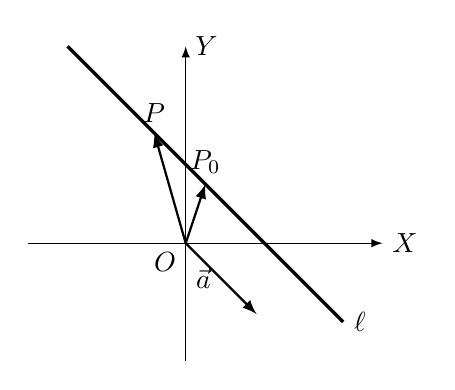
\begin{tikzpicture}[>=latex]
    \draw[->](-2,0)--(2.5,0)node[right]{$X$}; 
\draw[->](0,-1.5)--(0,2.5)node[right]{$Y$};
\node at (0,0)[below left]{$O$};
\draw[domain=-1.5:2, samples=10, very thick]plot(\x, {-\x+1})node[right]{$\ell$};
\draw[thick,->](0,0)--node[left]{$\vec{a}$}(.9,-.9);
\draw[thick,->](0,0)--(-.4,1.4)node[above]{$P$};
\draw[thick,->](0,0)--(.25,.75)node[above]{$P_0$};
\end{tikzpicture}
    \caption{}
\end{figure}


这就是说,直线$\ell$上的
点可以和实数$t$建立一一对
应关系.

一般来说,在取定的坐标系中,如果曲线上任一点的坐
标$x,y$都是某个变数$t$的函数时,
\begin{equation}
    x=f(t),\qquad y=\varphi(t)
\end{equation}
并且对于$t$的每一允许值,由方程(7.8)所确定的点$P(x,y)$
都在这条曲线上.那么方程(7.8)就叫做这条\textbf{曲线的参数方
程}.例如,方程(7.7)就是通过$P_0(x_0,y_0)$且平行于已知
向量$\vec{a}$的直线的参数方程.

上面我们用参数来表示直角坐标系中点的坐标$x,y$, 
同样我们也可用参数来表示在极坐标系中,点的极坐标$r,
\theta$. 即
\[  r=f(t),\qquad \theta=\varphi(t)\]

相对于参数方程来说,直接给出点的坐标间的关系的曲
线方程,叫做曲线的\textbf{普通方程}.如我们学过的直角坐标方程
和极方程.

\subsection{曲线的参数方程}
除上节建立的直线参数方程外,现在我们来建立几种常
见的曲线的参数方程.

\subsubsection{圆的参数方程}


以原点为圆心,$R$为半
径的圆,可以看作是一个质
点作等速圆周运动的轨迹
(图7.12).设质点的运
动的角速度为$\omega$, 从圆周与
$X$轴的正半轴的交点$A$的位
置开始按逆时针方向运动,
经过时间$t$后,质点到达圆周上一点$P(x,y)$的位置.由于
$\angle AOP=\omega t$,所以
\begin{equation}
    \begin{cases}
    x=R\cos\omega t\\
    y=R\sin\omega t
    \end{cases}
\end{equation}
在方程(7.9)中,对应$t$的每一个值,圆周上就有一点
$P(x,y)$与它对应.当$t$的值从0逐渐增加到
$2\pi/\omega$时,$P$
点就从$A$点开始按逆时针方向描出一个圆,所以(7.9)式就
是表示以原点为中心,$R$为半径的圆的参数方程.如果直接
取$\angle AOP=\theta$作为参数,那么圆的参数方程是
\[  \begin{cases}
    x=R\cos\theta\\
    y=R\sin\theta
    \end{cases}\]

\begin{figure}[htp]\centering
    \begin{minipage}[t]{0.48\textwidth}
    \centering
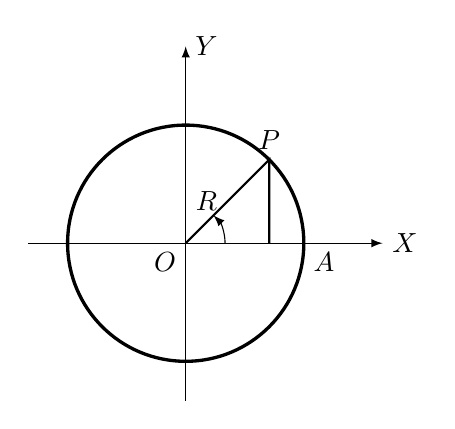
\begin{tikzpicture}[>=latex, scale=1]
\draw[->](-2,0)--(2.5,0)node[right]{$X$}; 
\draw[->](0,-2)--(0,2.5)node[right]{$Y$};
\node at (0,0)[below left]{$O$};
\draw[very thick](0,0) circle (1.5);
\draw[thick](0,0)--node[left]{$R$}(45:1.5)node[above]{$P$}--(1.06,0);
\node at (1.5,0)[below right]{$A$};
\draw[->](.5,0) arc (0:45:.5);  
    \end{tikzpicture}
    \caption{}
    \end{minipage}
    \begin{minipage}[t]{0.48\textwidth}
    \centering
    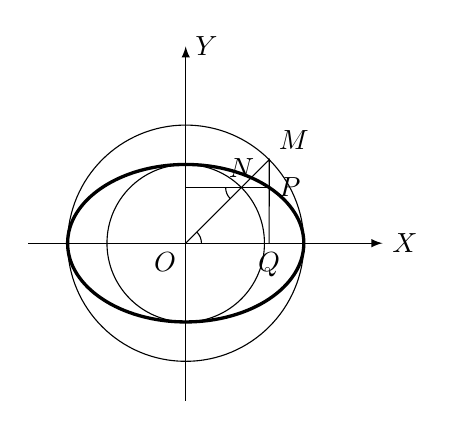
\begin{tikzpicture}[>=latex, scale=1]
\draw[->](-2,0)--(2.5,0)node[right]{$X$}; 
\draw[->](0,-2)--(0,2.5)node[right]{$Y$};
\node at (0,0)[below left]{$O$};
\draw(0,0) circle (1.5);
\draw(0,0) circle (1);
\draw[very thick] (0,0) ellipse [x radius=1.5, y radius=1];
\draw(0,.707)--(1.06,.707)node[right]{$P$};
\draw(0,0)--(45:1.5)node[above right]{$M$}--(1.06,0)node[below]{$Q$};

\tkzDefPoints{1.06/0/Q, 1.06/.707/P, 1.06/1.06/M, .707/.707/N}
\tkzDrawPoints(Q,P,M,N)
\node at (45:1)[above]{$N$};

\draw(.2,0) arc (0:45:.2);
\draw(.707-.2,.707) arc (180:180+45:.2);
    \end{tikzpicture}
    \caption{}
    \end{minipage}
    \end{figure}


\subsubsection{椭圆的参数方程}
    设$P(x,y)$是椭圆
$\frac{x^2}{a^2}+\frac{y^2}{b^2}=1$上任一点,以$O$为圆心,
分别以$a,b$为半径作两个辅助圆(图7.13).
过$P$点作直线$PQ$垂直于
$X$轴,垂足为$Q$点,并交大
辅助圆于$M$点,作$\overline{OM}$.

设$\angle MOX\varphi$,则$x=\overline{OQ}=a\cos\varphi$.
把上式代入椭圆方程,得$y=b\sin\varphi$,因此:
\begin{equation}
    \begin{cases}
        x=a\cos\varphi\\
        y=b\sin\varphi     
    \end{cases}
\end{equation}
就是椭圆的一个参数方程,其中$\varphi$叫做\textbf{离心角}.

\subsubsection{双曲线的参数方程}

由三角公式
\[\sec^2\varphi-\tan^2\varphi=1\]
我们可得双曲线$\frac{x^2}{a^2}-\frac{y^2}{b^2}=1$的一个参数方程为
\begin{equation}
    \begin{cases}
        x=a\sec\varphi\\
       y=b\tan\varphi
    \end{cases}
\end{equation}

\subsubsection{抛物线$y^2=2px$的参数方程}

如果令$y=2pt$,则$x=2pt^2$,所以
\begin{equation}
    \begin{cases}
        x=2pt^2\\ y=2pt
    \end{cases}
\end{equation}
可作为抛物线$y^2=2px$的一个参数方程.

\subsubsection{旋轮线的参数方程}
一个半径是$a$的车轮,沿一条直线轨道滚动,轮周上一
点$P$的轨迹叫做\textbf{旋轮线}(图7.14).
\begin{figure}[htp]
    \centering
	\begin{tikzpicture}[scale=1]
		\coordinate (O) at (0,0);
		\coordinate (Y) at (0,3);
		\def\r{1.5} % radius
		\def\p{1}
		\coordinate (B) at (\r, \r);
		\coordinate (A) at (\r, 0);
		\coordinate (P) at ({\r * (\p - sin(\p*180/pi))}, {\r * (1 - cos(\p*180/pi))});
		
		\draw[-latex] (0,-0.5) -- (Y) node[anchor=west] {$Y$};
		\draw[-latex] (-0.5,0) -- (2.4*pi*\r,0) node[anchor=west] {$X$};
		\draw[domain=0:{2*pi},samples=50,variable=\t] plot ({\r * (\t - sin(\t*180/pi)))},{\r * (1 - cos(\t*180/pi)))});
		\draw (B) circle (\r);
		\draw (B)--(A) (B)--(0,\r) coordinate (F);
		\draw (P) -- ({\r*(\p - sin(\p*180/pi))}, 0) coordinate (D);
		\draw (P) -- (\r, {\r*(\p * (1- cos(\p*180/pi)))}) coordinate (C);
		\draw (P) -- (B);
		
		\tkzLabelPoint[below left](O){$O$}
		\tkzLabelPoints[below](D,A)	
		\tkzLabelPoints[right](B,C)
		\tkzLabelPoints[above](P)
		\tkzMarkAngle[size=0.3](P,B,A) \tkzLabelAngle[pos=0.5](P,B,A){$\varphi$};
		\tkzLabelSegment(B,F){$a$}
	\end{tikzpicture}
    \caption{}
\end{figure}

下面我们来建立旋轮线的参数方程.

取$P$点落在轨道上的个一位置作为原点.轨道所在直线
作为$X$轴,当车轮从开始起转过了$\varphi$角,设这时$P$点的坐标
是$(x,y)$, 车轮的圆心在$B$点,与轨道相切于$A$点,于
是$\wideparen{AP}$的长等于$\overline{OA}$的长,我们引入参数$\varphi$(弧度).(叫
做滚动角)来表示$x$和$y$.

作$PD\bot OX$于$D$点,$PC\bot BA$于$C$点,则
\[\begin{split}
    x&=\overline{OD}=\overline{OA}-\overline{DA}=\wideparen{AP}-\overline{PC}=a\varphi-a\sin\varphi=a(\varphi-\sin\varphi)\\
    y&=\overline{DP}=\overline{AC}=\overline{AB}-\overline{BC}=a -a\cos\varphi=a(1-\cos\varphi)
\end{split}\]
因此,$P$点的轨迹的参数方程是
\begin{equation}
    \begin{cases}
        x=a(\varphi-\sin\varphi)\\
        y=a(1-\cos\varphi)
    \end{cases}
\end{equation}
(7.13)式就是旋轮线的一个参数方程.

\subsubsection{圆的渐开线参数方程}

把一条没有伸缩性的绳子绕在一个固定的圆盘的侧面
上,拉开绳子的一端并拉直,使绳子和圆周始终相切,然后
逐渐展开.绳子端点的轨迹叫做圆的\textbf{渐开线}(图7.15).
这个圆叫做渐开线的\textbf{基圆}.
\begin{figure}[htp]
    \centering
	\begin{tikzpicture}[scale=1]
		\coordinate (O) at (0,0);
		\coordinate (Y) at (0,3.5);
		\def\r{1} % radius
		\def\p{1.2	}
		\coordinate (A) at (\r, 0);
		\pgfmathsetmacro{\u}{\r*(cos(\p*180/pi)+\p*sin(\p*180/pi))}
		\pgfmathsetmacro{\v}{\r * (sin(\p*180/pi) - \p*cos(\p*180/pi))}
		\coordinate (B) at (\u,\v);
		
		\draw[-latex] (0,-1.5) -- (Y) ;
		\draw[-latex] (-1.6*pi*\r,0) -- (2	*\r,0) ;
		\draw[domain=0:{4.49341},samples=50,variable=\t] plot ({\r*(cos(\t*180/pi)+\t*sin(\t*180/pi))},{\r * (sin(\t*180/pi) - \t*cos(\t*180/pi))});
		\draw (O) circle (\r);
		
		\pgfmathsetmacro{\uvsqsum}{\u * \u + \v * \v}
		\pgfmathsetmacro{\Cx}{(\u - \v * sqrt(\uvsqsum - 1)) / \uvsqsum}
		\pgfmathsetmacro{\Cy}{sqrt(1 - \Cx * \Cx)}
		\coordinate (C) at (\Cx,\Cy);
		\draw (B)--(C)--(O)--(B);
		\tkzMarkAngle[size=0.3](A,O,B)
		\tkzLabelSegment[above](O,C){$a$}
		\tkzLabelSegment[above=-0.1](O,B){$r$}
		\tkzMarkRightAngle(O,C,B)
		\tkzLabelPoints[below right](A)
		\tkzLabelPoints[right](B)
		\tkzLabelPoints[above](C)
		\tkzLabelPoints[below left](O)
	\end{tikzpicture}
    \caption{}
\end{figure}

下面我们来建立渐开线的参数方程.

设定圆的圆心为$O$, 半径为$a$, 开始时绳子的外端在$A$
点,$O$为极点,以射线$OA$
为极轴建立极坐标系,设$B$
是渐开线上任一点,$(r,\theta)$是
它的极坐标,其中$\theta$的单位
是弧度.$\overline{OA}=a$, 
$\angle BOC=\alpha$, 则$r=\frac{a}{\cos\alpha}$,
$\overline{BC}=a\tan\alpha$. 根据题设应有
\[\overline{BC}=\wideparen{AC}=a(\alpha+\theta)\]
解出$\theta$, 得
\[\theta=\frac{\overline{BC}}{a}-\alpha=\tan\alpha-\alpha\]
因此,渐开线的极坐标的参数方程为
\begin{equation}
    \begin{cases}
        r=\frac{a}{\cos\alpha}\\
    \theta=\tan\alpha-\alpha
    \end{cases}
\end{equation}

以$OA$为$X$轴的正半轴,建立直角坐标系.
取$\angle AOC=\varphi$ 作为参数,由于
$\varphi =\alpha+\theta$, 
应用公式(7.14)式的第二式可得
$$\varphi  =\tan\alpha$$
设$B$点在$OXY$中的坐标为$(x,y)$, 则
\begin{equation}
\begin{split}
    x&=r\cos\theta=a(\cos\varphi+\varphi\sin\varphi)\\
    y&=r\sin\theta=a(\sin\varphi-\varphi\cos\varphi)
\end{split}
\end{equation}
这是渐开线在直角坐标系中的参数方程.

由以上几种常见曲线的参数方程的推导可知,通常建立
曲线的参数方程有两种方法:一种是像(一)那样,把曲线
看作动点的轨迹,选取时间参数$t$, 使得曲线上的点的动坐
标$x,y$分别用$t$的函数来表示,另一种是像(二)、(三)那
样,从已知曲线的直角坐标方程引入适当的参数,从而求得
曲线的参数方程.最后,我们指出,一条曲线的参数方程不
是唯一的.

以后我们将会看到,利用参数方程研究曲线的形状和性
质比普通方程更加方便.

\begin{example}
    画出参数方程$\begin{cases}
        x=t^2\\ y=t^3
    \end{cases}$
    所表示的曲线.
\end{example}


\begin{solution}
列表
\begin{center}
\begin{tabular}{ccccccccc}
\hline
$t$&$\cdots$ &$-3$ &$-2$&0&1&2&3&$\cdots$\\
\hline
$x$&$\cdots$ & 9&4&0&1&4&9             &$\cdots$ \\
$y$&$\cdots$ & $-27$&$-8$ &0&1&8&27  &$\cdots$ \\
\hline
\end{tabular}
\end{center}

用表中的数对$(x,y)$描点作图,就可
得到方程的曲线(图7.16).这条曲线叫做\textbf{半立方抛物线}.

\begin{figure}[htp]
    \centering
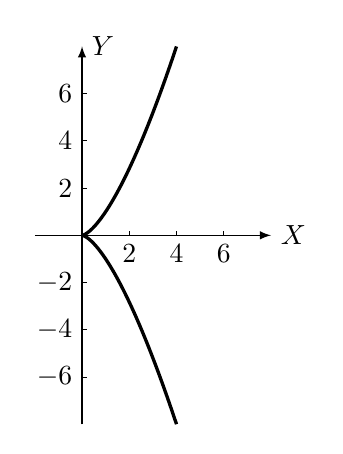
\begin{tikzpicture}[>=latex, scale=.3]
\draw[->](-2,0)--(8,0)node[right]{$X$};
\draw[->](0,-8)--(0,8)node[right]{$Y$};
\draw[domain=0:4, samples=100, very thick]plot(\x, {\x*sqrt(\x)});
\draw[domain=0:4, samples=100, very thick]plot(\x, {-\x*sqrt(\x)});
\foreach \x in {2,4,6}
{
   \draw(0,\x)node[left]{\x}--(.2,\x);
   \draw(\x,0)node[below]{\x}--(\x,.2);
}
\foreach \x in {-2,-4,-6}
{
   \draw(0,\x)node[left]{$\x$}--(.2,\x);
}


\end{tikzpicture}
    \caption{}
\end{figure}

\end{solution}

\begin{ex}
\begin{enumerate}
    \item 写出下列直线的参数方程.
\begin{enumerate}
    \item 过$P(2,3)$且平行于已知向量$\vec{a}=(1,4)$的
    直线
    \item 过$P_1(3,4)$, $P_2(4,-3)$两点的直线
    \item $y=kx$
    \item $y=kx+b$
\end{enumerate}
\item 一质点沿方向$\vec{S}=\left(\cos\frac{\pi}{6},\sin\frac{\pi}{6}\right)$, 
从点$P_0(1,2)$, 
以3m/s的速率运动,写出运动轨迹的参数方程.
\item 已知一条直线上两点$M_1(x_1,y_1)$, $M_2(x_2,y_2)$, 以
分点$M(x,y)$分$\overline{M_1M_2}$所成的比$\lambda$为参数.写出这条直线的参数方程.
\item 已知抛物线$x=2pt^2$, $y=2pt$, 写出通过对应于参数
$t_1,t_2$两点的弦的方程.
\item 作下列参数方程的图形.
\begin{enumerate}
\item $x=t$, $y=3t$
\item $x=3\sin\theta$, $y=4\cos\theta$
\item $x=4t^2$, $y=2t$
\end{enumerate}
\end{enumerate}
\end{ex}

\subsection{参数方程和普通方程的互化}
设曲线的参数是
\[\begin{cases}
   x=f(t)\\
y=\varphi(t) 
\end{cases}\]
如果我们能从这个方程消去参数$t$, 那么我们就可求出当线
的普通方程.
 
\begin{example}
    把参数方程$\begin{cases}
        x=5\cos t+2\\
y=2\sin t-3
    \end{cases}$化为普通方程.
\end{example}

\begin{solution}
    由已知参数方程可得
\[\frac{x-2}{5}=\cos t,\qquad \frac{y+3}{2}=\sin t\]
两式两边平方后相加,得
\[\frac{(x-2)^2}{25}+\frac{(y+3)^2}{4}=1\]
这就是已知曲线的普通方程.
\end{solution}

\begin{example}
    把参数方程
\begin{numcases}{}
    x=at^2\\
    y=a^2t^3
\end{numcases}
化为普通方程.
\end{example}

\begin{solution}
(7.16)式两边立方,(7.17)式两边平方,得
\begin{align}
    x^3=a^3t^6\\
    y^2=a^4t^6
\end{align}
由(7.18), (7.19)两式可得
\[y^2=ax^3\]
\end{solution}

\begin{example}
    化直线的点斜式方程$y-y_0=k(x-x_0)$为参数
方程.
\end{example}

\begin{solution}
    直线的点斜式方程可变为
\[kx-y+y_0-kx_0=0\]
因此直线具有方向向量为$\vec{S}=(1,k)$, 所以,直线方程的
参数方程可写为
\[\begin{cases}
    x=x_0+t\\ y=y_0+kt
\end{cases}\]
\end{solution}




\begin{ex}
\begin{enumerate}
    \item 把下列曲线的参数方程化为普通方程.
    \begin{multicols}{2}
\begin{enumerate}
    \item $\begin{cases}
        x=3+2t\\y=2-3t
    \end{cases}$
    \item $\begin{cases}
        x=2+3\cos\theta\\
        y=4-3\sin\theta
    \end{cases}$
    \item $\begin{cases}
        x=t\\y=4t^2
    \end{cases}$
    \item $\begin{cases}
        x=\cos^2 t\\ y=\sin t
    \end{cases}$
\end{enumerate}
    \end{multicols}

\item 把下列普通方程化为参数方程.
\begin{multicols}{2}
\begin{enumerate}
    \item $\frac{x-2}{4}=\frac{x+5}{3}$
    \item $y=4x$
    \item $\frac{(x-h)^2}{a^2}+\frac{(y-k)^2}{b^2}=1$
    \item $\frac{(x-h)^2}{a^2}-\frac{(y-k)^2}{b^2}=1$
    \item $y=6x^2$
    \item $y^2=8x$
\end{enumerate}
\end{multicols}
\end{enumerate}
\end{ex}

\section*{习题7.2}
\addcontentsline{toc}{subsection}{习题7.2}

\begin{enumerate}
\item 已知直线$\ell$通过点$P_0(x_0,y_0)$并且与已知单位向量
$\vec{e}=(\cos\alpha,\sin\alpha)$平行,求直线$\ell$的参数方程.
\item 求经过点$P(1,3)$, 倾角是$\pi/4$
的参数方程.
\item 已知$M(x,y)$从原点以常速度向量$\vec{v}(v_x,v_y)$运动.
求$M$点的轨迹的参数方程.并且把它化为普通方程.如
果$M$点从$A(a,b)$点开始运动,$M$点的轨迹的参数方
程怎样?
\item 把下列参数方程化成普通方程.
\begin{multicols}{2}
\begin{enumerate}
    \item $\begin{cases}
        x=t^2-2t\\y=t^2+2
    \end{cases}$
    \item $\begin{cases}
        x=\frac{a(1-t^2)}{1+t^2}\\
        y=\frac{2bt}{1+t^2}
    \end{cases}$
    \item $\begin{cases}
        x=a\sec\varphi\\
        y=b\tan\varphi
    \end{cases}$
    \item $\begin{cases}
        x=5t^2-1\\y=10t^2+4
    \end{cases}$
    \item $\begin{cases}
        x=\frac{a}{2}\left(t+\frac{1}{t}\right)\\
        y=\frac{b}{2}\left(t-\frac{1}{t}\right)
    \end{cases}$
\end{enumerate}
\end{multicols}
\item 已知抛物线$x=2pt^2$, $y=2pt$, 求证:通过对应$t_1$,
$t_2$两点的直线方程是
\[x-(t_1+t_2)y+2pt_1t_2=0\]
\item 已知抛物线$x=2pt^2$, $y=2pt$, 求证:抛物线在点$t_1$
处的切线方程为
\[x-2t_1y+2pt_1^2=0\]
\item 求证:抛物线$x=2pt^2$, $y=2pt$, 在点$t_1$、$t_2$处的切
线交点的坐标是
\[\big(2pt_1t_2,\; p(t_1+t_2)\big)\]
\item 利用第7题的结论,证明:抛物线通过焦点的弦的两个端
点处的切线相交在准线上.

\end{enumerate}

\section*{复习题七}
\addcontentsline{toc}{section}{复习题七}

\begin{enumerate}
    \item 画出下列各极坐标方程的图形.
\begin{multicols}{2}
    \begin{enumerate}
        \item $r\theta =a$
        \item $r=2\theta$
        \item $r=5(1-\cos\theta )$
        \item $r=a\sin3\theta$
        \item $r=a\cos\theta +b$
        \item $r^2=16\sin 2\theta$
    \end{enumerate}
\end{multicols}

\item 把下列各曲线的极坐标方程化为直角坐标方程.
\begin{multicols}{2}
\begin{enumerate}
\item $r\sin\theta =10$
\item $r=4\sin\theta$
\item $r(5+3\cos\theta )=16$
\item $r(4+5\cos\theta )=9$
\item $r^2\cos2\theta =-1$
\item $r(\sin\theta +2\cos\theta )=6$
\item $r=2\cos\theta +3\sin\theta $
\item $\theta =45^{\circ}$
\item $r=\frac{3}{2+3\sin\theta}$ 
\item $r^2=9\cos2\theta $
\end{enumerate}
\end{multicols}

\item 把下列各直角坐标方程化为极坐标方程.
\begin{multicols}{2}
  \begin{enumerate}
\item $\frac{x^2}{a^2}-\frac{y^2}{b^2}=1$
\item $\frac{x^2}{a+x}=\frac{y^2}{a-x}$
\item $x^2+y^2=3xy$
\item $y^2=\frac{x^3}{2a-x}$
\item $x^2+y^2+2Dx+2Ey+F=0$
\item $(x^2+y^2)^3=4x^2y^2$
\item $x^4+x^2y^2-(x+y)^2=0$
\item $(x^2+y^2)^3=16x^2y^2(x^2-y^2)^2$
\end{enumerate}  
\end{multicols}


\item 说明下列两条直线的位置关系.
\begin{enumerate}
    \item $\theta =\alpha$ 和$r \cos(\theta-\alpha)=a$ ($a>0$且为定值);
\item $\theta =\alpha$ 和$r\sin(\theta -\alpha)=a$.
\end{enumerate}

\item 求证:经$P(r_1,\theta_1)$点和极轴交成$\alpha$角的直线方程是
\[r\sin(\theta -\alpha )=r_1\sin(\theta_1-\alpha)\]
\item $O$点是原点,$P$点是椭圆$x=3\cos\varphi$, $y=2\sin\varphi$上相
当于$\varphi=\pi/6$的一点,求直线$OP$的倾角.
\item 已知椭圆
$x=a\cos\varphi$, $y=b\sin\varphi$, 求证:通过对应
$\varphi =\alpha$和$\varphi =\beta$ 椭圆上两点的直线方程是
\[\frac{x}{a}\cos\frac{1}{2}(\alpha+\beta )+\frac{y}{b}\sin\frac{1}{2}(\alpha+\beta )=\cos\frac{1}{2}(\alpha-\beta )\]
\item 已知椭圆$x=a\cos\varphi$, $y=b\sin\varphi$. 求证:椭圆上对应
$\varphi_1$点的切线方程是
\[\frac{x}{a}\cos\varphi_1+\frac{y}{b}\sin\varphi_1=1\]
\item 一个圆的圆心在$C(a,b)$, 半径为$R$. 求这个圆以圆
心角$\theta$(从$X$轴的正方向算起)为参数的参数方程.
\item 已知$P$、$Q$是椭圆
$x=a\cos\varphi$, $y=b\sin\varphi$ 上分别对应
$\varphi_1$和$\varphi_2$的两点.求证:直线$OP$和$OQ$为椭圆共轭直
径的条件是$|\varphi_1-\varphi_2|=90^{\circ}$.
\item 已知椭圆$x=a\cos\varphi$, $y=b\sin\varphi$, $P$、$Q$是椭圆上对
应$\varphi$ 和$\varphi +90^{\circ}$的两点,求证:
\[|\Vec{OP}|^2+|\Vec{OQ}|^2=a^2+b^2\]

\item 画出下列参数方程表示的图形.
\begin{multicols}{2}
\begin{enumerate}
    \item $\begin{cases}
        x=3t-5\\y=t^3-t
    \end{cases}$
    \item $\begin{cases}
        x=t-\sin t\\ y=1-\cos t
    \end{cases}$
\end{enumerate}
\end{multicols}
\end{enumerate}


